 \section{van der Meer calibration}
\label{sec:vdm}
Van der Meer (vdM) scans are done to calculate the visible cross section $\sigma_{vis}$ of the pixel detector which is a calibration constant in the relation between rate of a quantity (clusters, coincidences) read out by the detector and the instantaneous luminosity. \\

The instantaneous luminosity  per bunch crossing when the crossing angle between the colliding bunches is negligible and bunches collide head on as shown in Fig. 7 is given by the following integral, \cite{CMS-PAS-LUM-13-001} \\

$L_{inst/bunch}$ = N_1 N_2 f \int^{+\infty}_{-\infty} \rho_1(x,y) \rho_2(x+\Delta x, y+ \Delta y) dx dy \\

where $N_1, N_2$ are the number of protons in the colliding bunches, f is the LHC orbit frequency whose value is 11246Hz,  $\rho_1(x,y)$ and $\rho_2(x+\Delta x,y+\Delta y)$ are the two dimensional particle density distribution functions for each colliding bunch separated by $\Delta x$ and $\Delta y$ in the x and y directions. \\

Assuming complete factorization of particle density distribution function along x and y directions for both the bunches, we get \\

$L_{inst/bunch}$ = N_1 N_2 f \int^{+\infty}_{-\infty} \rho_{1x}(x) \rho_{2x}(x+\Delta x)  dx   \int^{+\infty}_{-\infty} \rho_{1y}(y) \rho_{2y}(y+\Delta y)  dy \\

where $\rho_1(x,y) = \rho_{1x}(x,y) \rho_{1y} (x,y)$ and $\rho_2(x+\Delta x,y + \Delta y) = \rho_{2x}(x+\Delta x,y+\Delta y) \rho_{2y} (x+\Delta,y+\Delta y)$ \\

The vdM scan determines the bunch  overlap integrals $\int \rho_{x1} (x) \rho_{x2} (x+\Delta x) dx$ and  $\int \rho_{y1}(y) \rho_{y2} (y+\Delta y) dy$ by measuring pixel clusters rate as a function of bunch separation $\Delta x$ and $\Delta y$ along x and y directions as shown in Fig. 8. \\

\int \rho_{x1} (x) \rho_{x2} (x+\Delta x) dx = \frac{R_x(0)}{\int R_x(\Delta x)dx} \\

\int \rho_{y1} (y) \rho_{y2} (y + \Delta y) dy = \frac{R_y(0)}{\int R_y(\Delta y)dy} \\

where $R_x(0)$ is the measured cluster rate along x direction when the bunch separation is zero and $R_x(\Delta x)$ is the measured cluster rate when bunches are separated by distance $\Delta x$ and $R_y(0)$ is the measured cluster rate along y direction when the bunch separation is zero and $R_y(\Delta y)$ is the measured cluster rate when bunches are separated by distance $\Delta y$. \\

Bunch overlap widths $\Sigma_x$ and $\Sigma_y$ along x and y directions are defined as \\

\Sigma_x = \frac{1}{\sqrt{2 \pi}} \frac{\int R_x(\Delta x)dx}{R_x(0)} \\

\Sigma_y =  \frac{1}{\sqrt{2 \pi}} \frac{\int R_y(\Delta y)dy}{R_y(0)} \\

$\Sigma_x \Sigma_y = \frac{1}{2 \pi} \frac{\int R_x(\Delta x)dx \int R_y(\Delta y) dy}{R_x(0) R_y(0)}$  is the bunch overlapping area as shown in Fig. 9 by the red region.\\

Thus, the expression for instantaneous luminosity is given by \\

$L_{inst/bunch}$ = $\frac{N_1 N_2 f}{2\pi \Sigma_x \Sigma_y}$ \\

and the PCC visible cross section defined in terms of beam parameters and rate is given by \\

\sigma_{vis} = \frac{2 \pi \Sigma_x \Sigma_y R}{N_1 N_2} \\

where R = $\frac{d}{dt} <N_{cluster}>$  is cluster rate.\\

\begin{figure}[H]
  \centering
  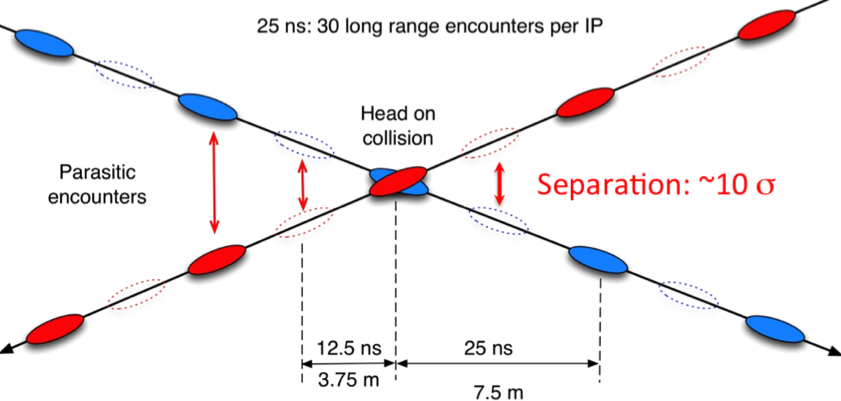
\includegraphics[width=0.6\columnwidth]{./LHCReport_1_image_cut.png}
  \caption{ \onehalfspacing Diagram showing colliding bunches in each LHC beam separated by 25ns.}
  \label{fig:CMS}
\end{figure}




\begin{figure}[H]
  \centering
  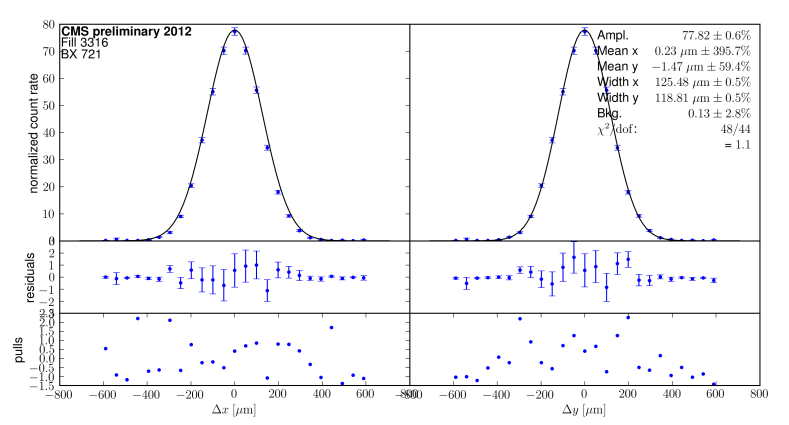
\includegraphics[width=0.7\columnwidth]{./vdm_ratefit.png}
  \caption{ \onehalfspacing Cluster rate profile fit during vdM scans as a function of bunch separation $\Delta x$ and $\Delta y$ along x and y directions. \cite{CMS-PAS-LUM-15-001}.}
  \label{fig:CMS}
\end{figure}


\begin{figure}[H]
  \centering
  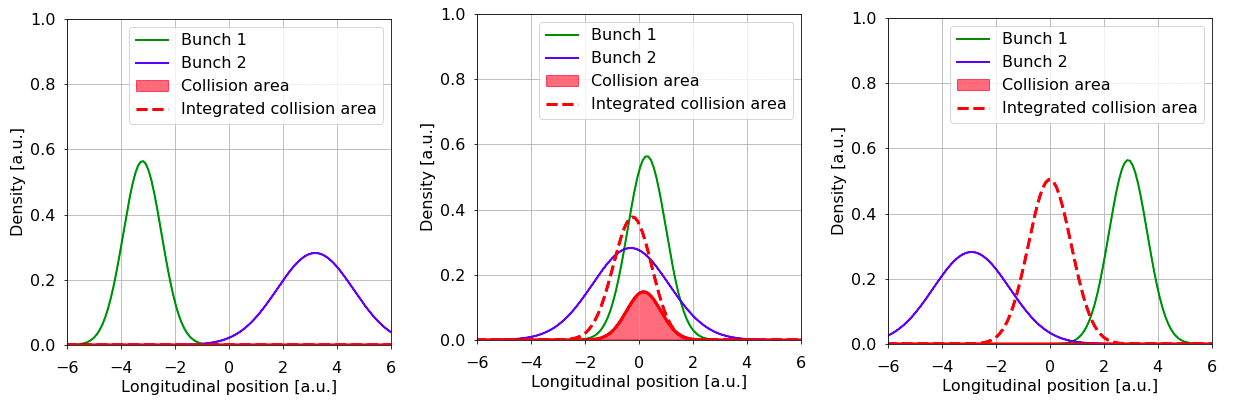
\includegraphics[width=\columnwidth]{./vdm_image.png}
  \caption{\onehalfspacing Figure showing two LHC bunches in green and blue approaching each other and colliding giving rise to an overlapping region showing in red whose area is determined during vdM scans.}
  \label{fig:CMS}
\end{figure}






